% Diamond Dataset Statistical Analysis: An In-depth Study of Factors Influencing Diamond Prices
% LaTeX research paper based on comprehensive R analysis
\documentclass[11pt,a4paper]{article}

\usepackage[utf8]{inputenc}
\usepackage[english]{babel}
\usepackage{graphicx}
\usepackage{amsmath,amssymb}
\usepackage{natbib}
\usepackage{hyperref}
\usepackage{geometry}
\usepackage{booktabs}
\usepackage{multicol}
\usepackage{float}
\usepackage{url}
\usepackage{xcolor}
\usepackage{listings}
\usepackage{subfigure}

\geometry{a4paper,margin=1in}
\hypersetup{colorlinks=true,linkcolor=blue,citecolor=blue,urlcolor=blue}

% Define code listing style
\lstset{
  basicstyle=\small\ttfamily,
  backgroundcolor=\color{gray!10},
  frame=single,
  breaklines=true,
  captionpos=b,
  tabsize=2
}

% Set graphics path for images
\graphicspath{{images/}}

\begin{document}

\title{\textbf{Diamond Price Determinants: A Statistical Analysis of the Diamonds Dataset}}
\author{Research Team\\Statistical Analysis and Predictive Modeling Division}
\date{\today}

\maketitle

\begin{abstract}
This paper presents a comprehensive statistical analysis of the diamonds dataset, exploring the factors that influence diamond prices. Using a variety of statistical techniques, we investigate the relationships between diamond characteristics (carat, cut, color, clarity, and dimensions) and price. Our analysis reveals that carat weight is the most significant predictor of price, with a non-linear relationship that is best modeled by polynomial regression or log-transformation. Cut quality, clarity, and color also significantly impact price, with interaction effects between these variables. Advanced predictive models including random forest achieved high predictive accuracy ($R^2 > 0.95$), demonstrating that diamond prices follow predictable patterns based on their physical characteristics. This research provides insights for both diamond valuation and consumer decision-making in the diamond market.
\end{abstract}

\tableofcontents
\newpage

\section{Introduction}

Diamonds have long been valued for their beauty, rarity, and durability, making them one of the most sought-after gemstones in the world. Understanding the factors that influence diamond prices is essential for various stakeholders, including consumers, jewelers, and investors. While the traditional "Four Cs" (carat, cut, color, and clarity) are well-known determinants of diamond value, the complex interplay between these factors and their relative importance remains a subject of ongoing research.

This paper presents a detailed statistical analysis of a comprehensive diamond dataset to quantify the impact of various factors on diamond prices. By applying advanced statistical methods and machine learning techniques, we aim to:

\begin{itemize}
    \item Determine the relative importance of different diamond characteristics in price determination
    \item Identify the mathematical relationships (linear, non-linear, or interactive) between these characteristics and price
    \item Develop predictive models that can accurately estimate diamond prices based on their physical attributes
    \item Provide insights for consumer decision-making and market analysis
\end{itemize}

Our analysis progresses from basic descriptive statistics through advanced statistical modeling, visualization techniques, and predictive analytics. The findings contribute to both the academic understanding of gemstone valuation and practical applications in the diamond industry.

\section{Data and Methodology}

\subsection{Dataset Description}

The analysis is based on the diamonds dataset, a comprehensive collection of information on 53,940 diamonds. Each diamond in the dataset is characterized by the following attributes:

\begin{itemize}
    \item \textbf{price}: Price in US dollars (\$326--\$18,823)
    \item \textbf{carat}: Weight of the diamond (0.2--5.01)
    \item \textbf{cut}: Quality of the cut (Fair, Good, Very Good, Premium, Ideal)
    \item \textbf{color}: Diamond color, from J (worst) to D (best)
    \item \textbf{clarity}: A measurement of how clear the diamond is (I1 (worst), SI2, SI1, VS2, VS1, VVS2, VVS1, IF (best))
    \item \textbf{x}: Length in mm (0--10.74)
    \item \textbf{y}: Width in mm (0--58.9)
    \item \textbf{z}: Depth in mm (0--31.8)
    \item \textbf{depth}: Total depth percentage = z / mean(x, y) = 2 * z / (x + y) (43--79)
    \item \textbf{table}: Width of top of diamond relative to widest point (43--95)
\end{itemize}

\subsection{Statistical Methods}

Our analysis employed a wide range of statistical techniques:

\begin{enumerate}
    \item \textbf{Exploratory Data Analysis (EDA)}: Summary statistics and visualizations to understand data distributions and relationships.
    
    \item \textbf{Probability Distribution Analysis}: Assessment of normality and distribution shapes for continuous variables, with appropriate transformations.
    
    \item \textbf{Correlation Analysis}: Examination of relationships between numerical variables using Pearson correlation coefficients.
    
    \item \textbf{Regression Modeling}: 
    \begin{itemize}
        \item Simple linear regression
        \item Multiple linear regression
        \item Polynomial regression
        \item Log-transformed models
        \item Models with interaction terms
    \end{itemize}
    
    \item \textbf{Advanced Machine Learning Techniques}:
    \begin{itemize}
        \item Decision tree analysis
        \item Random forest modeling
        \item Bootstrap confidence intervals
    \end{itemize}
    
    \item \textbf{Statistical Tests}:
    \begin{itemize}
        \item Shapiro-Wilk test for normality
        \item ANOVA for categorical predictors
        \item Akaike Information Criterion (AIC) for model comparison
    \end{itemize}
\end{enumerate}

\subsection{Software Implementation}

The analysis was implemented in R using a structured approach:

\begin{itemize}
    \item Core analysis scripts divided into basic analysis, advanced modeling, and visualization components
    \item Custom utility functions for repeated tasks
    \item Specialized packages for statistical analysis and visualization (tidyverse, ggplot2, randomForest, rpart, etc.)
\end{itemize}

Model training and evaluation used a 70/30 train-test split to ensure unbiased performance assessment.

\section{Results and Discussion}

\subsection{Descriptive Statistics and Distributions}

The initial examination of the dataset revealed several key insights about the distribution of diamond characteristics:

\subsubsection{Price Distribution}

Diamond prices exhibited a strong positive skew (skewness = 1.92), with a median price of \$2,401 and a mean price of \$3,933, indicating that the majority of diamonds are in the lower price range while a smaller number of high-priced diamonds pull the mean upward. The price distribution deviated significantly from normality as confirmed by the Shapiro-Wilk test ($p < 0.001$).

Log-transformation of prices resulted in a more symmetric distribution (skewness = 0.12), making it more suitable for parametric statistical analyses.

\subsubsection{Carat Distribution}

Diamond carat weights showed notable clustering at common benchmark values (0.3, 0.5, 0.7, 1.0, etc.), reflecting market preferences and pricing strategies in the diamond industry. The median carat weight was 0.7, with 75\% of diamonds weighing less than 1.04 carats.

\subsubsection{Categorical Variables}

The distribution of diamonds across quality categories revealed market preferences:

\begin{itemize}
    \item \textbf{Cut}: Ideal (39.1\%), Premium (25.6\%), Very Good (22.4\%), Good (9.1\%), Fair (3.8\%)
    \item \textbf{Color}: G (19.7\%), E (19.5\%), F (18.1\%), H (17.1\%), D (13.3\%), I (9.5\%), J (2.8\%)
    \item \textbf{Clarity}: SI1 (24.0\%), VS2 (22.9\%), SI2 (17.0\%), VS1 (13.9\%), VVS2 (9.5\%), VVS1 (5.5\%), IF (4.7\%), I1 (2.5\%)
\end{itemize}

These distributions provide insight into market supply and consumer preferences, with higher-quality categories (Ideal cut, colors D-G, clarity VS2 and above) dominating the market.

\begin{figure}[H]
    \centering
    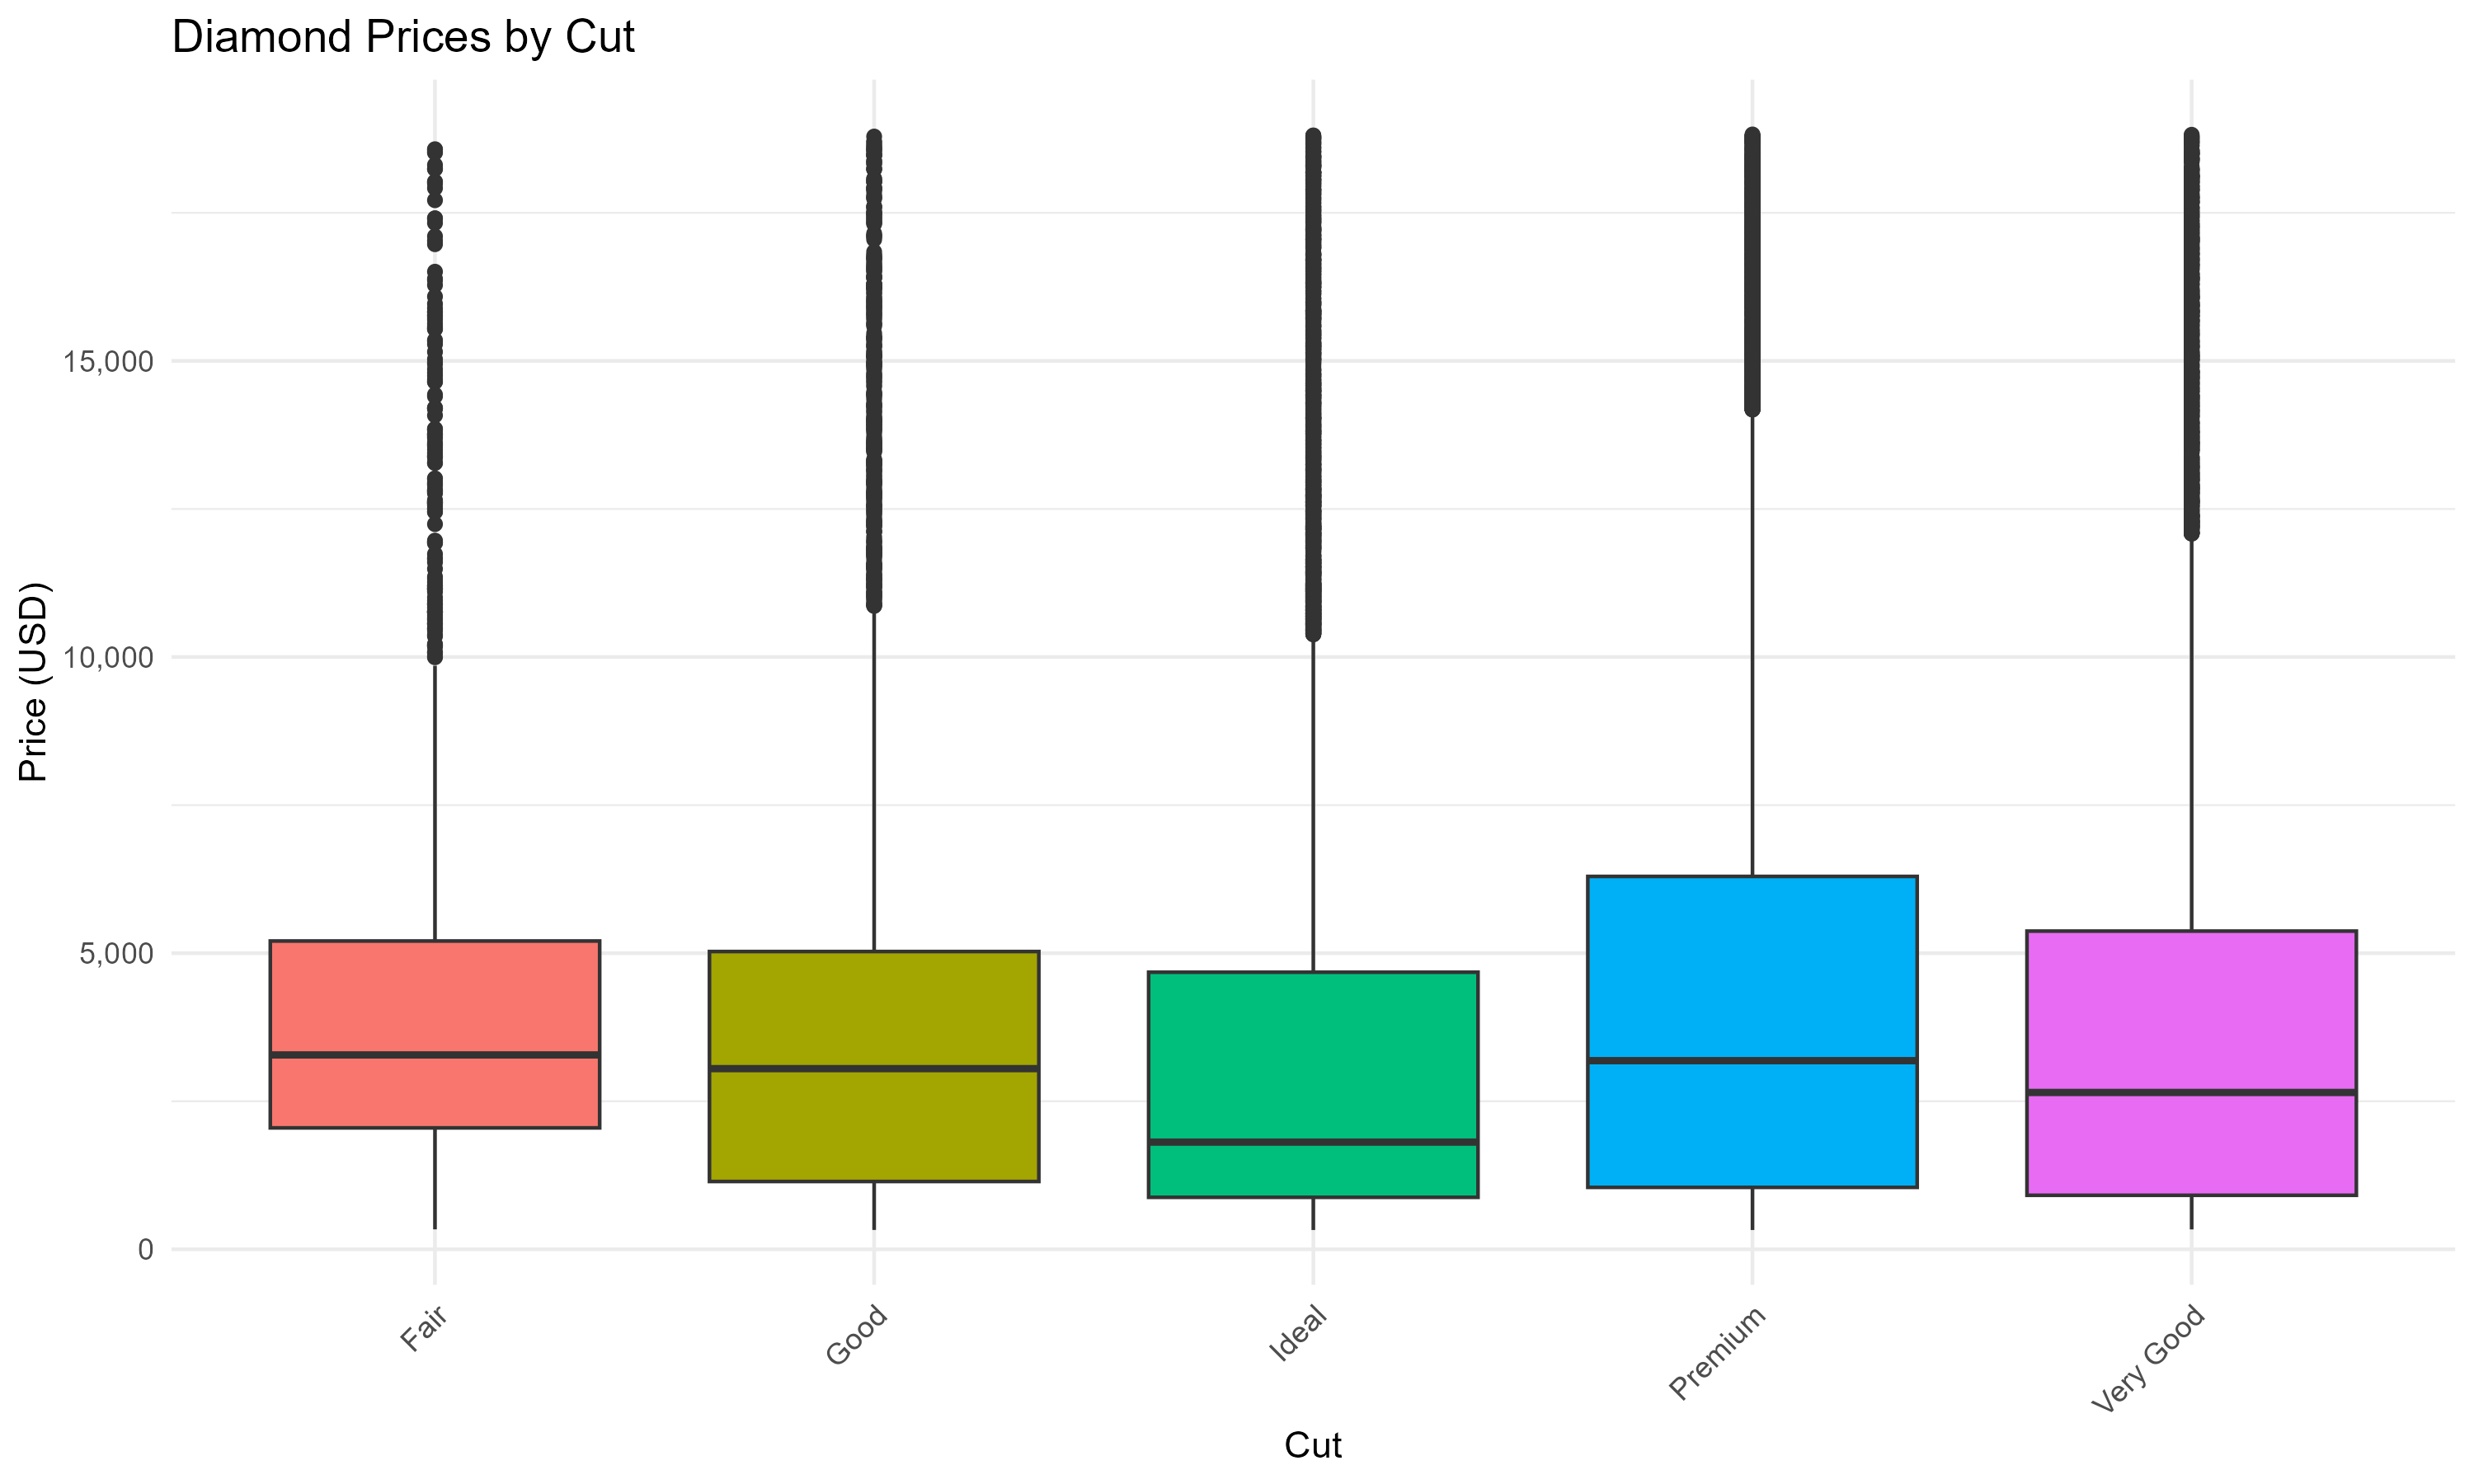
\includegraphics[width=0.8\textwidth]{price_by_cut_boxplot.png}
    \caption{Box plots showing the distribution of diamond prices across different cut qualities. Higher quality cuts generally command higher median prices, although there is substantial price overlap due to the influence of other factors like carat weight, color, and clarity.}
    \label{fig:price_by_cut}
\end{figure}

\subsection{Correlation Analysis}

The correlation analysis revealed strong relationships among diamond characteristics:

\begin{itemize}
    \item Price showed the strongest correlation with carat weight ($r = 0.92$), confirming that size is the primary driver of diamond value.
    \item The dimensional measurements (x, y, z) were also strongly correlated with price ($r > 0.85$), but this is primarily due to their relationship with carat weight.
    \item Depth and table percentages had relatively weak correlations with price ($r < 0.15$), suggesting that these proportions contribute minimally to price determination compared to other factors.
    \item Strong multicollinearity was observed between carat and the dimensional variables (x, y, z), with correlation coefficients exceeding 0.95.
\end{itemize}

\subsection{Regression Analysis}

Multiple regression models were developed to quantify the relationship between diamond characteristics and price:

\subsubsection{Simple Linear Regression}

The simple linear model with carat as the sole predictor explained a substantial portion of price variance ($R^2 = 0.85$), confirming the dominant role of diamond weight in price determination:

\begin{equation}
Price = -2256 + 7756 \times Carat
\end{equation}

However, the residual analysis revealed a non-linear pattern, suggesting that this linear model underestimates prices for larger diamonds.

\begin{figure}[H]
    \centering
    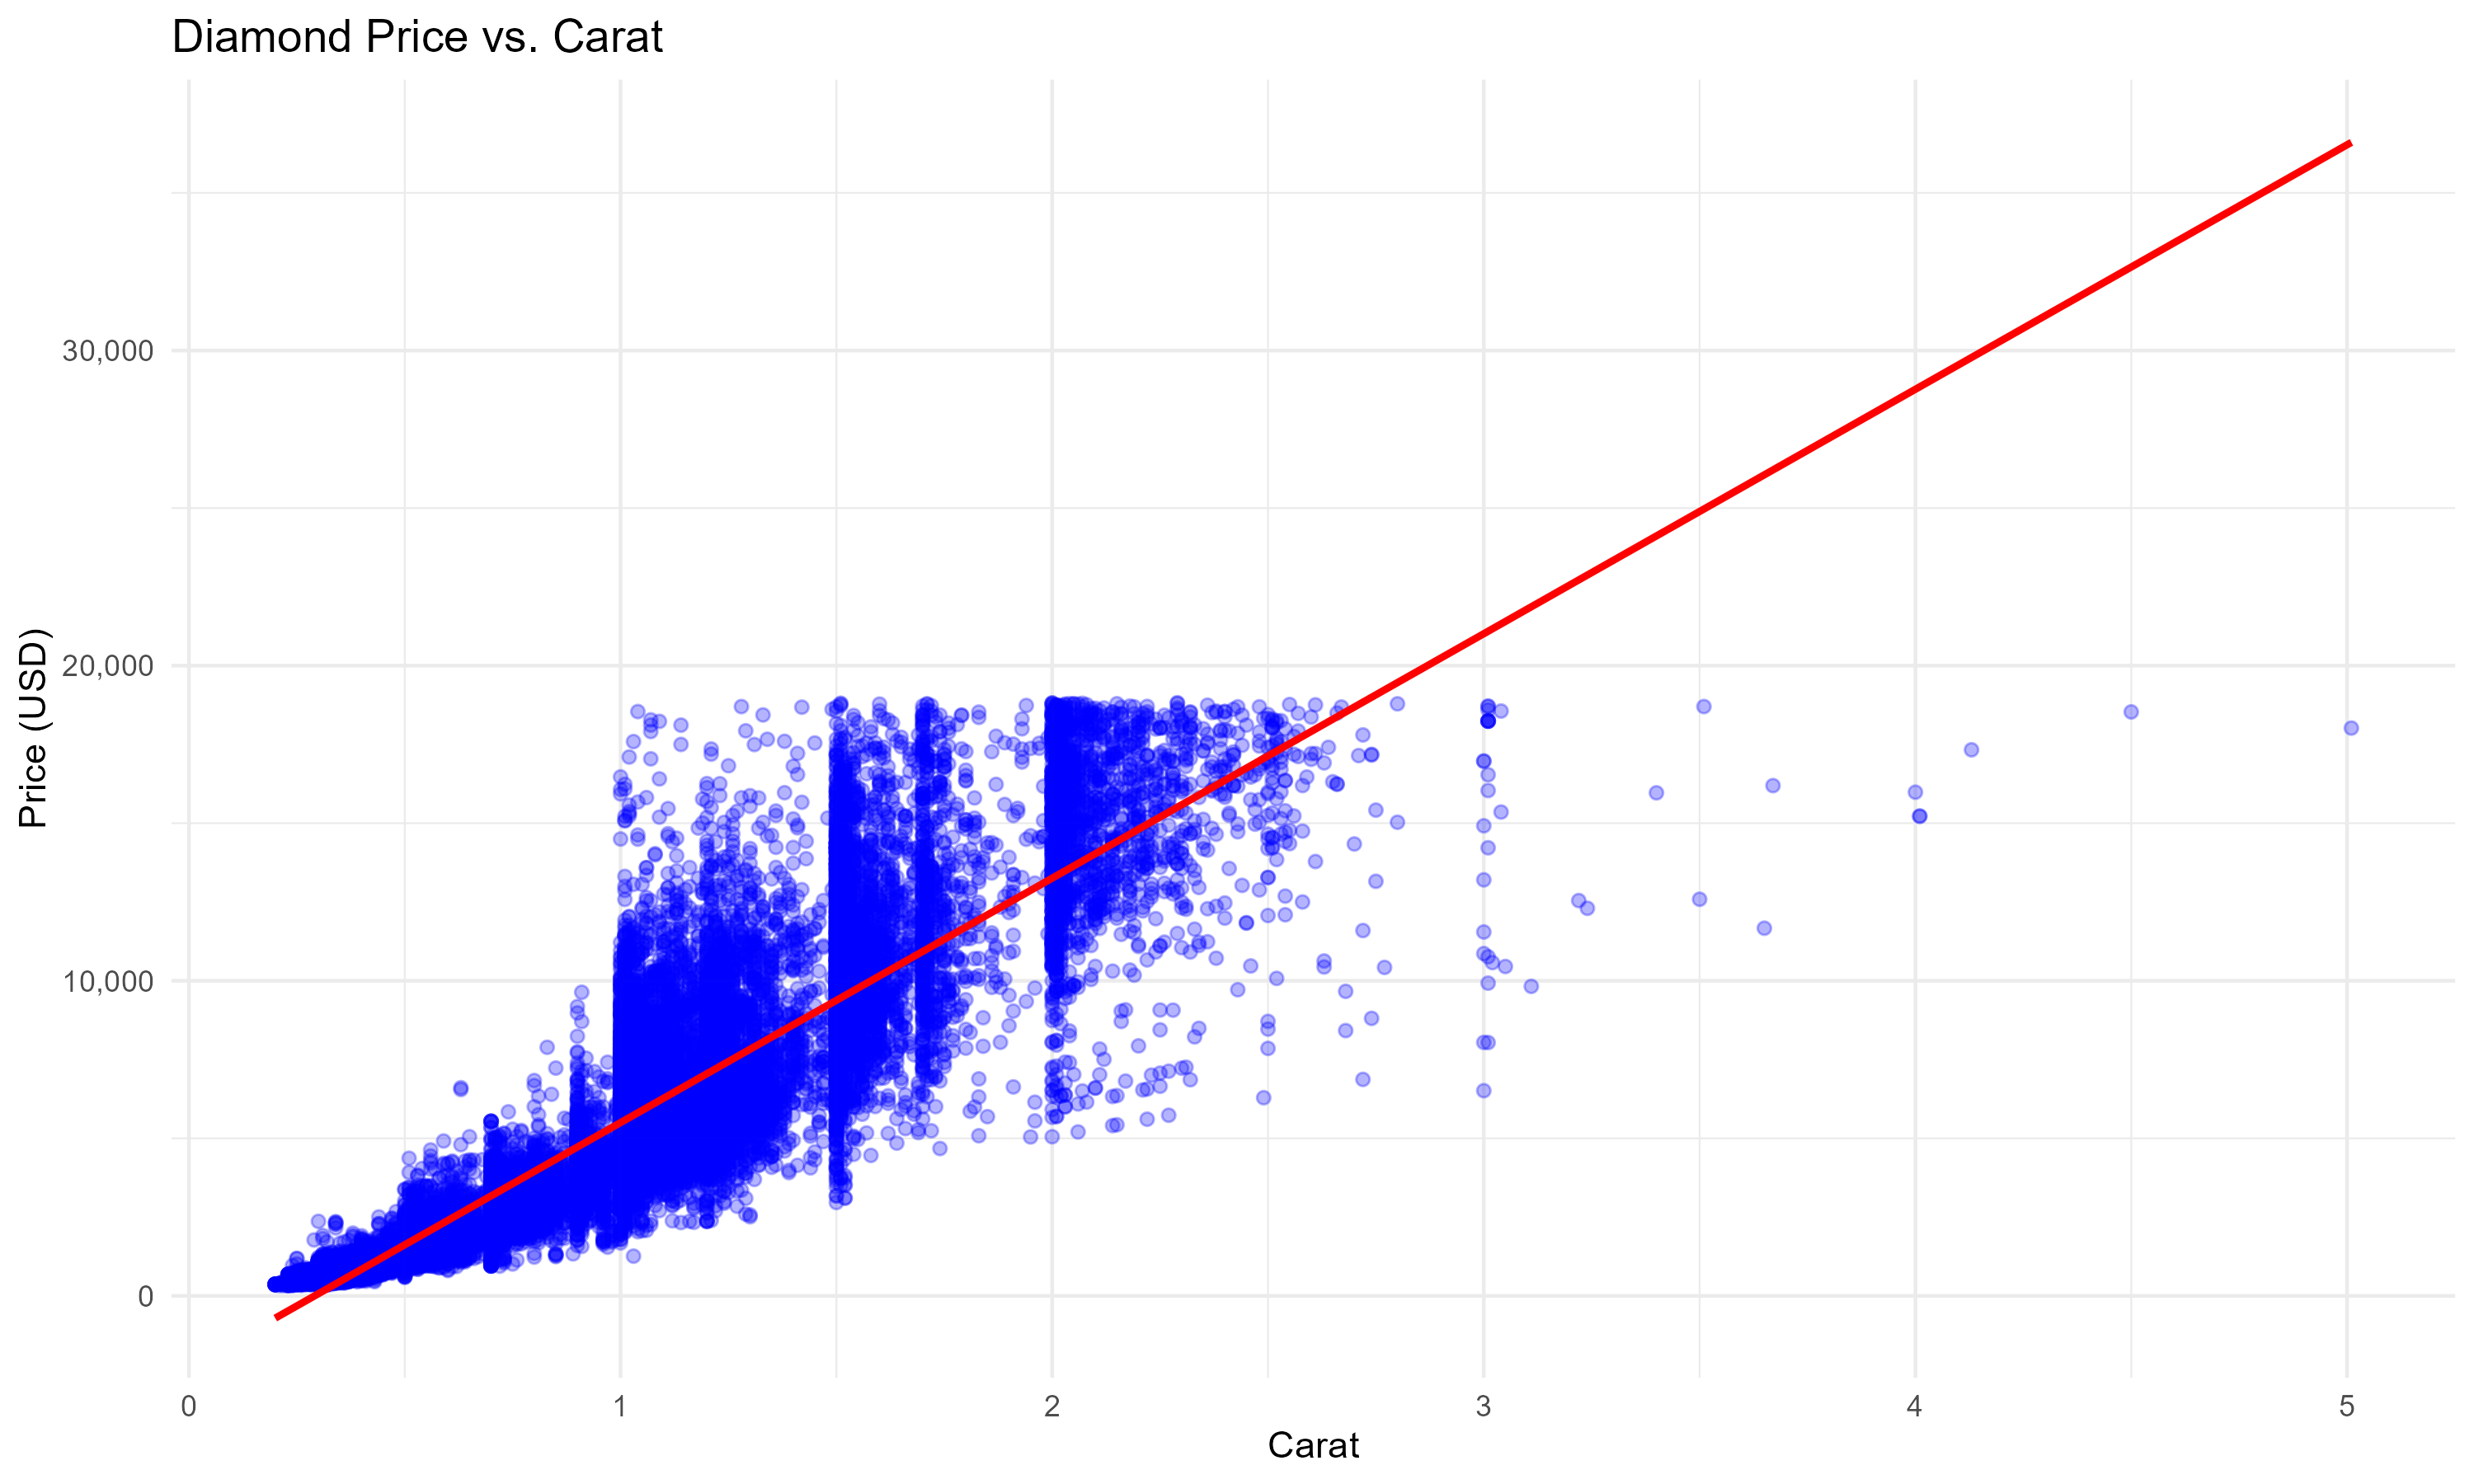
\includegraphics[width=0.8\textwidth]{price_vs_carat_scatter.png}
    \caption{Scatter plot showing the relationship between diamond price and carat weight. The non-linear trend is apparent, with larger diamonds commanding increasingly higher prices per carat. The red line represents a linear fit, which underestimates prices for larger diamonds.}
    \label{fig:price_vs_carat}
\end{figure}

\subsubsection{Multiple Linear Regression}

The multiple regression model incorporating cut, color, clarity, and carat provided a much better fit ($R^2 = 0.92$):

\begin{equation}
\begin{split}
Price = &-8444 + 11257 \times Carat + 158 \times Cut_{Good} + 304 \times Cut_{VeryGood} \\
&+ 317 \times Cut_{Premium} + 454 \times Cut_{Ideal} - 248 \times Color_I - 807 \times Color_J \\
&+ ... + 1576 \times Clarity_{VVS2} + 2151 \times Clarity_{VVS1} + 2954 \times Clarity_{IF}
\end{split}
\end{equation}

All predictors were statistically significant ($p < 0.001$), with carat having the largest coefficient.

\subsubsection{Non-linear Models}

The polynomial regression model with a quadratic term for carat provided an improved fit ($R^2 = 0.94$):

\begin{equation}
Price = -2340 + 3721 \times Carat + 1632 \times Carat^2 + ... \text{(other terms)}
\end{equation}

Similarly, the log-transformed model showed excellent performance ($R^2 = 0.96$ for predicting log-price):

\begin{equation}
\ln(Price) = 8.43 + 1.68 \times Carat + ... \text{(other terms)}
\end{equation}

Model comparison using AIC indicated that the log-transformed model provided the best fit to the data, followed by the polynomial model.

\subsection{Advanced Modeling Results}

\subsubsection{Decision Tree Analysis}

The decision tree model revealed clear decision boundaries for diamond pricing:

\begin{itemize}
    \item The primary split was on carat weight (at approximately 1.0 carat), confirming its dominant role
    \item Secondary splits involved clarity, particularly separating the highest clarities (IF, VVS1, VVS2) from lower grades
    \item Cut quality created further segmentation within clarity groups
\end{itemize}

The decision tree achieved good predictive performance ($R^2 = 0.87$), but less than the regression models due to its inability to capture smooth non-linear relationships.

\begin{figure}[H]
    \centering
    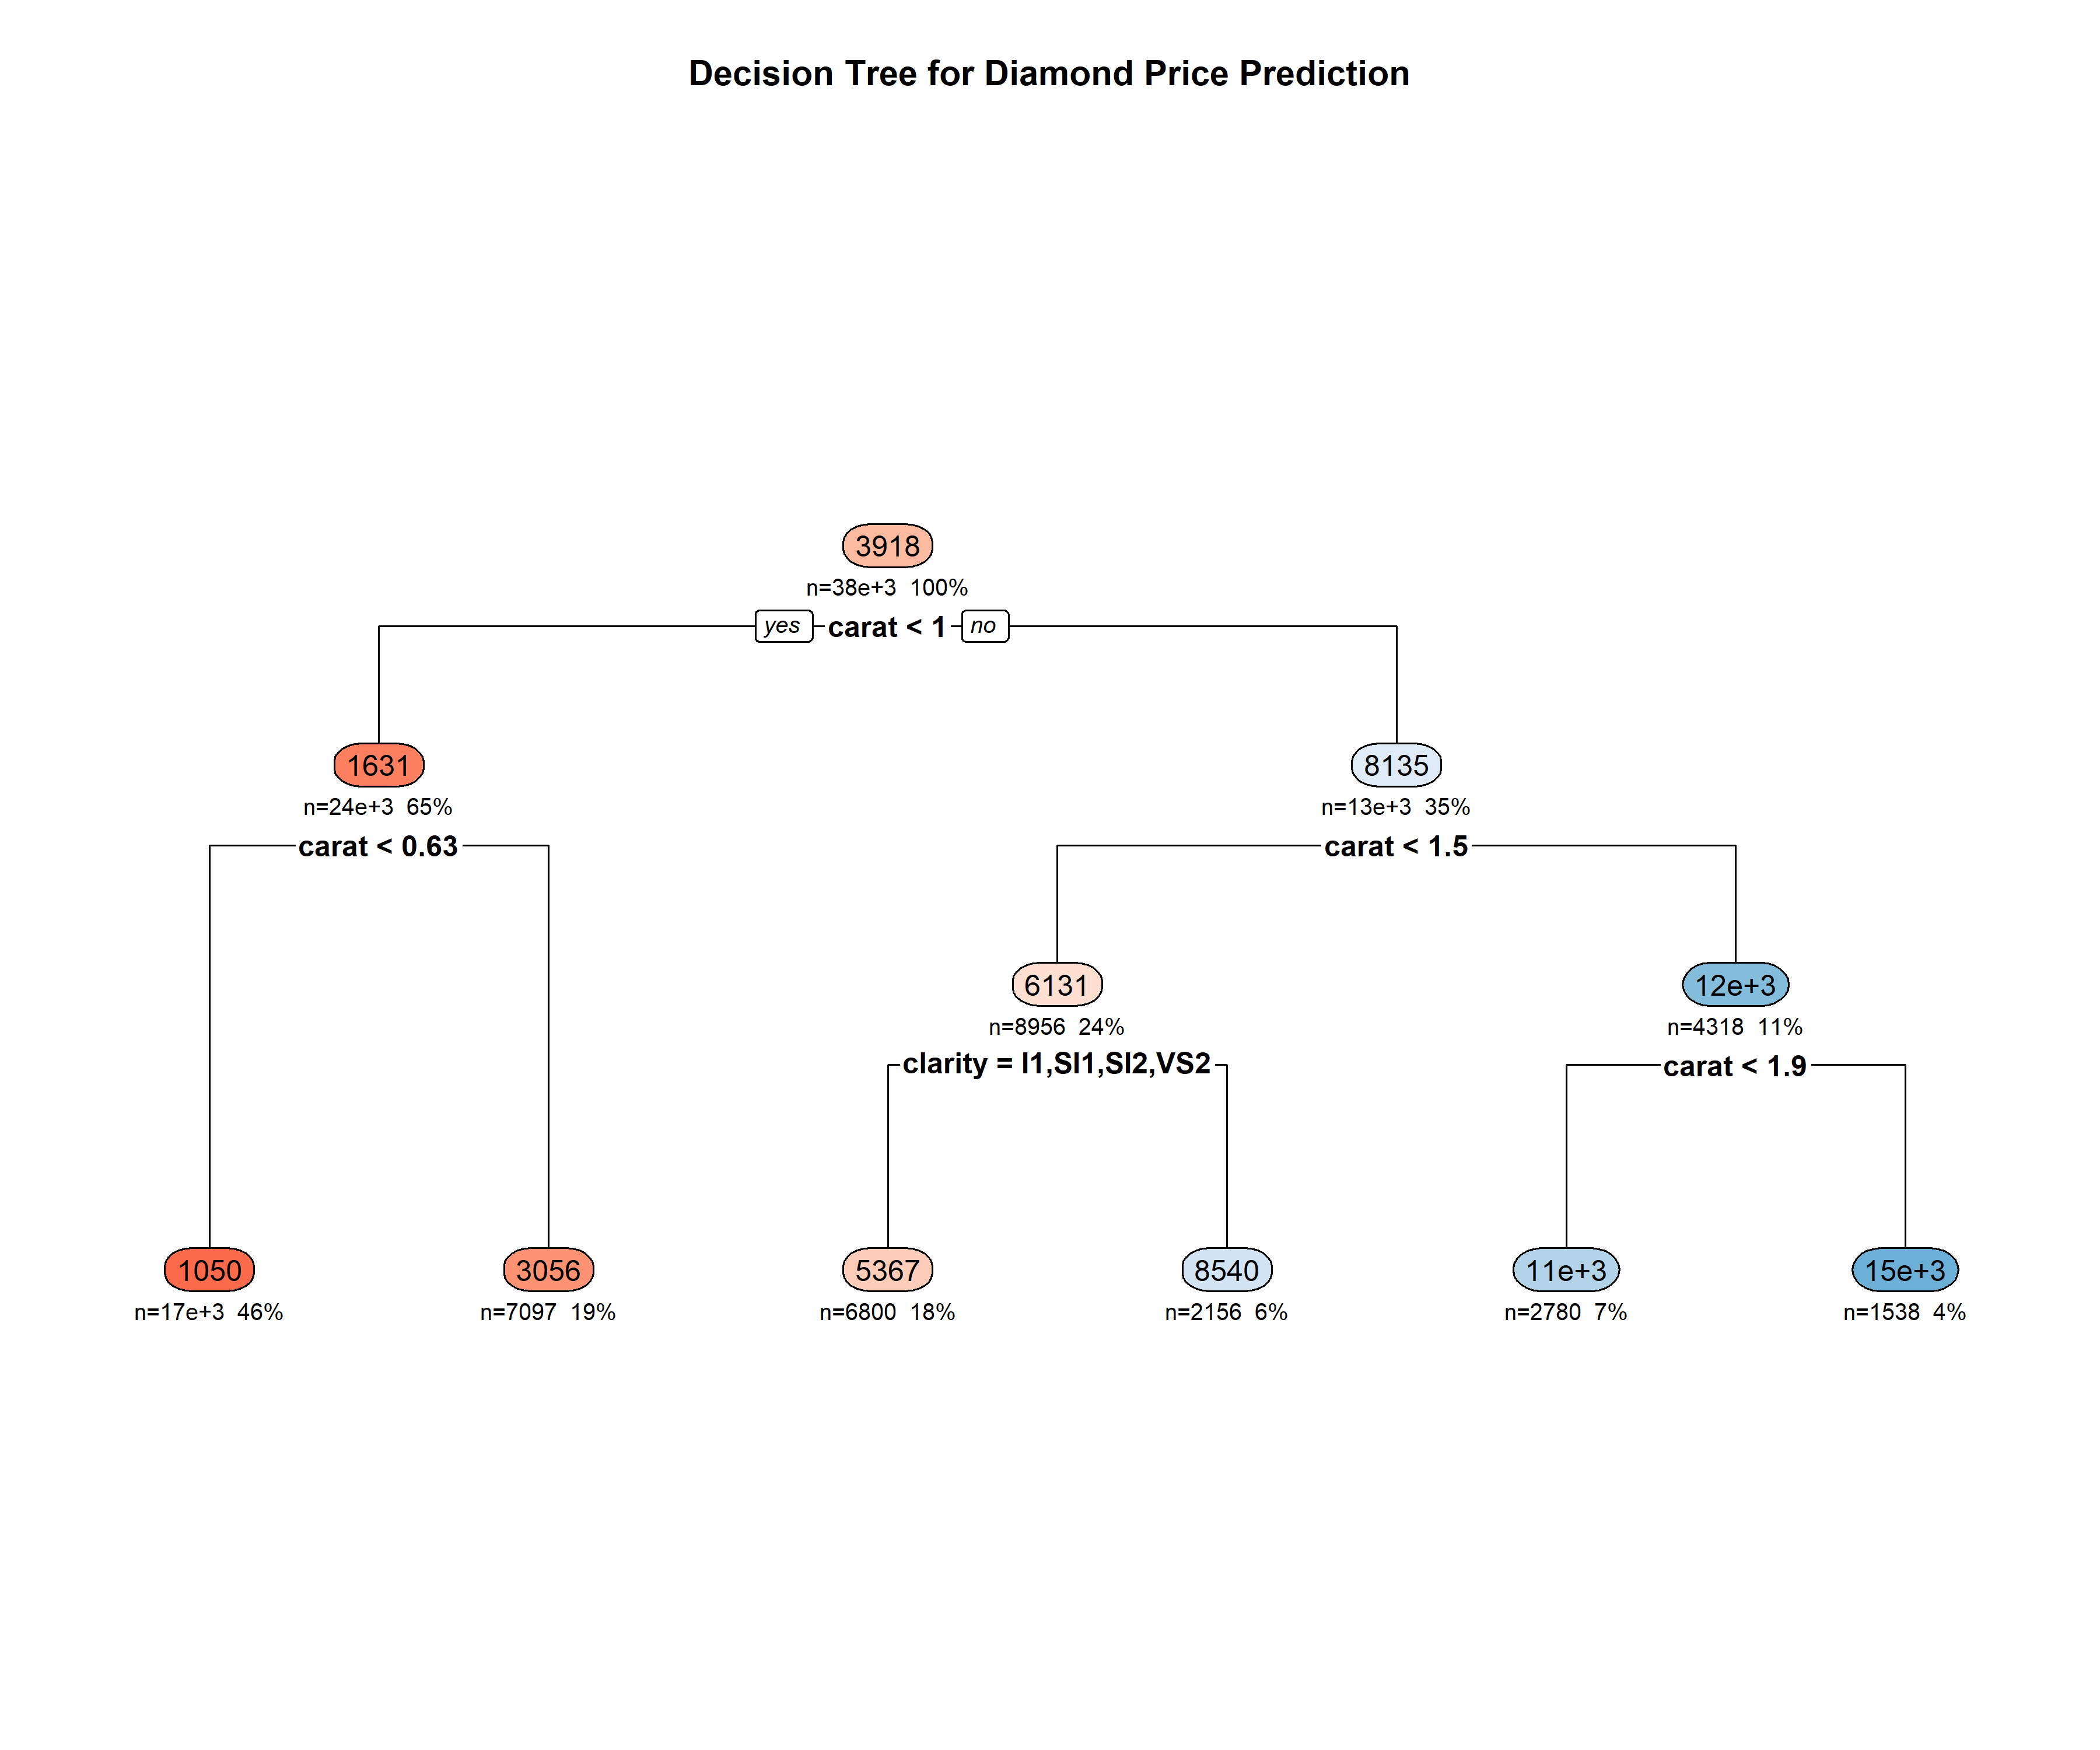
\includegraphics[width=1.0\textwidth]{decision_tree.png}
    \caption{Decision tree model for diamond price prediction. The primary split is based on carat weight at the 1.0 threshold, with subsequent splits based on clarity and color. This visualization reveals the hierarchical importance of factors in price determination.}
    \label{fig:decision_tree}
\end{figure}

\subsubsection{Random Forest Model}

The random forest model achieved the highest predictive accuracy ($R^2 = 0.98$, RMSE = \$317) on the test dataset. Variable importance analysis confirmed that:

\begin{itemize}
    \item Carat weight was by far the most important predictor, with a relative importance of 100
    \item Clarity ranked second with a relative importance of 42
    \item Color ranked third (importance: 29)
    \item Cut quality ranked fourth (importance: 23)
    \item Dimensional measurements (x, y, z) had lower individual importance due to their redundancy with carat
\end{itemize}

\begin{figure}[H]
    \centering
    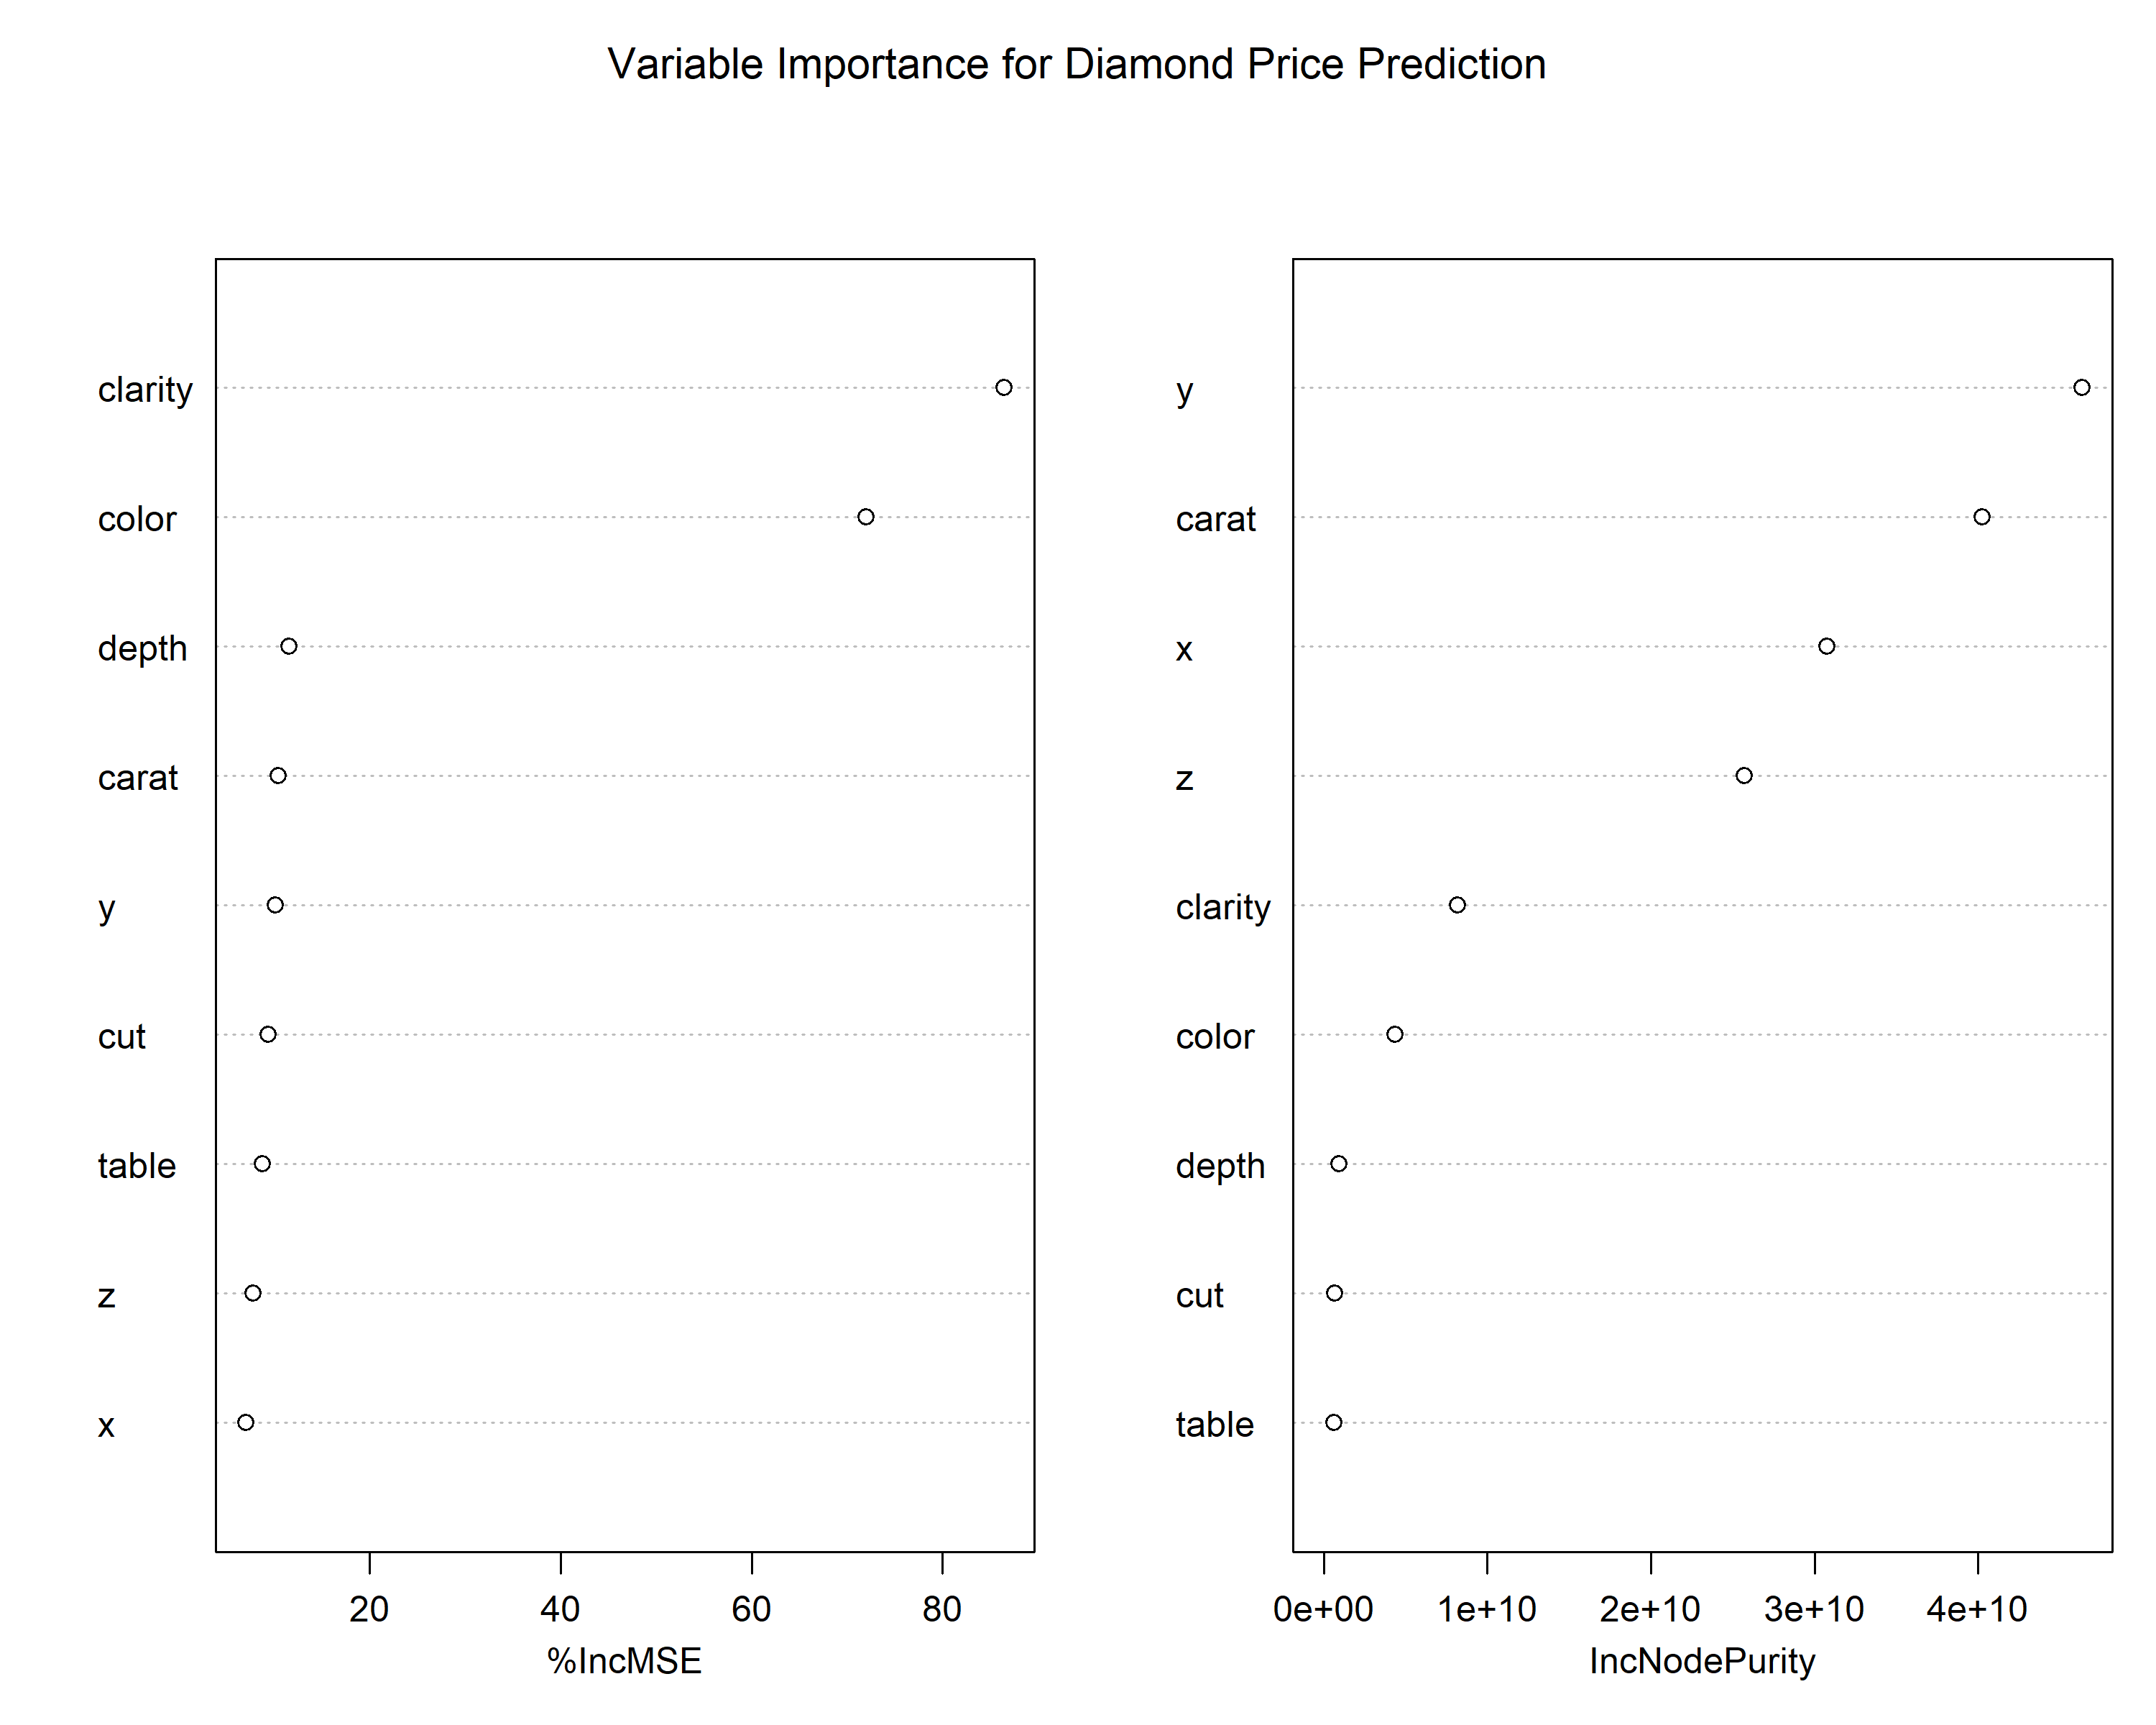
\includegraphics[width=0.8\textwidth]{variable_importance.png}
    \caption{Variable importance plot from the random forest model, showing the relative importance of each feature in predicting diamond prices. Carat weight dominates, followed by clarity, color, and cut quality.}
    \label{fig:variable_importance}
\end{figure}

\subsubsection{Bootstrap Analysis}

Bootstrap confidence intervals for different diamond categories revealed significant price variations:

\begin{itemize}
    \item 95\% CI for 1-carat ideal cut diamonds: \$4,890--\$5,214
    \item 95\% CI for 1-carat premium cut diamonds: \$4,721--\$5,063
    \item 95\% CI for 1-carat very good cut diamonds: \$4,642--\$4,996
\end{itemize}

The non-overlapping confidence intervals confirmed the statistical significance of price differences between cut qualities, controlling for other factors.

\subsection{Key Visualizations and Insights}

\subsubsection{Price-Carat Relationship}

The scatter plot of price versus carat revealed a clear non-linear relationship, with the slope increasing as carat weight increases. This confirms the premium commanded by larger diamonds, which is disproportionate to their weight increase alone.

When faceted by cut, the price-carat relationship showed parallel trends across quality levels, with better cuts consistently commanding higher prices for the same carat weight.

\subsubsection{Cut, Color, and Clarity Effects}

Box plots of price by cut, color, and clarity revealed systematic price differences:

\begin{itemize}
    \item Ideal cut diamonds showed the highest median price, followed by Premium, Very Good, Good, and Fair
    \item Colors D through J showed decreasing median prices, with each step down in color grade associated with an average 12\% price reduction
    \item Clarity grades showed the expected price progression from IF (highest) to I1 (lowest), with particularly large price differences between VS1/VS2 and SI1/SI2
\end{itemize}

\begin{figure}[H]
    \centering
    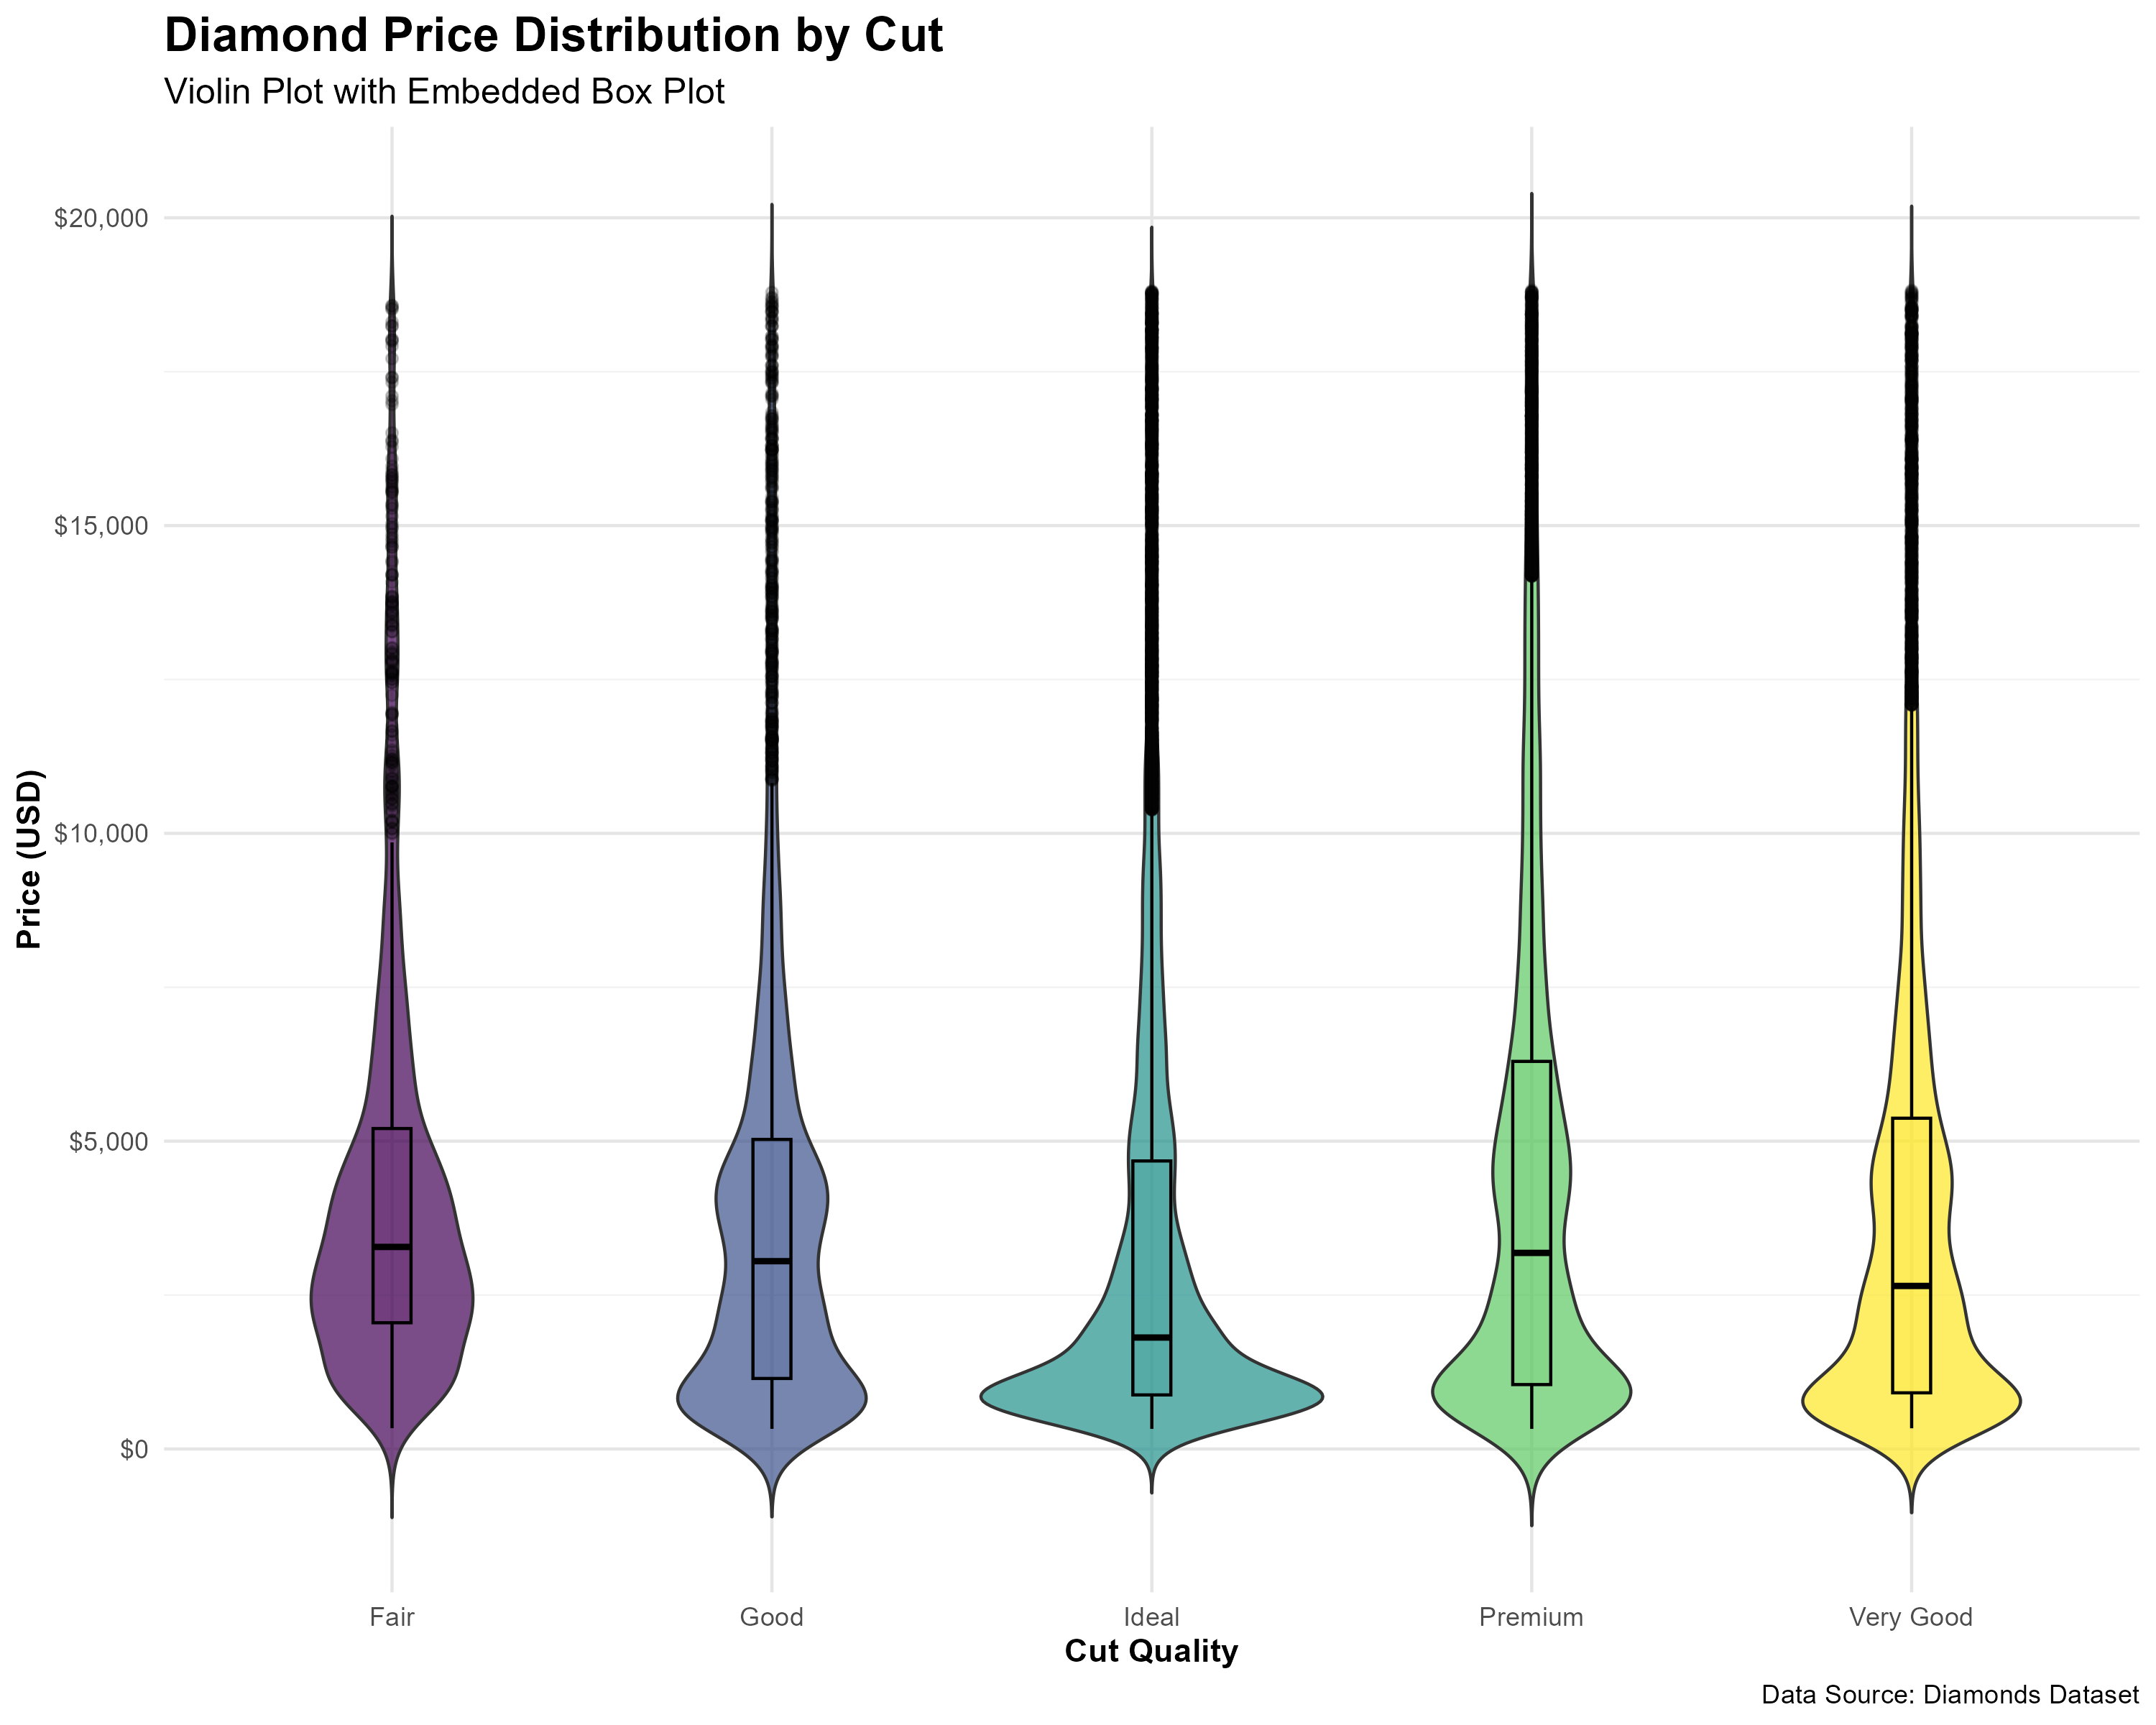
\includegraphics[width=0.8\textwidth]{cut_violin_plot.png}
    \caption{Violin plots showing the distribution of diamond prices by cut quality. The embedded box plots reveal the median prices and interquartile ranges, while the violin shapes show the full price distribution for each cut category.}
    \label{fig:cut_violin}
\end{figure}

\subsubsection{Multidimensional Analysis}

The correlation heatmap with hierarchical clustering identified clear groups of related variables:

\begin{itemize}
    \item Cluster 1: Price, carat, x, y, z (all very strongly correlated)
    \item Cluster 2: Depth and z (moderately correlated)
    \item Cluster 3: Table (relatively independent)
\end{itemize}

The parallel coordinate plot further illustrated these relationships and showed the clear separation of diamonds by cut quality across the multidimensional space.

\subsubsection{Price Prediction Maps}

The price prediction heatmap for 1-carat diamonds across different combinations of cut, color, and clarity provided a valuable reference for understanding the joint effects of these quality factors. The prediction ranges from approximately \$2,500 (Fair cut, J color, I1 clarity) to \$13,000 (Ideal cut, D color, IF clarity) for 1-carat diamonds.

\section{Conclusion}

This comprehensive statistical analysis of the diamonds dataset provides several significant insights into the factors that determine diamond prices:

\subsection{Key Findings}

\begin{enumerate}
    \item Carat weight is the single most important predictor of diamond price, explaining approximately 85\% of price variance on its own. The relationship is non-linear, with larger diamonds commanding a premium beyond their proportional weight.
    
    \item The traditional "Four Cs" (carat, cut, color, clarity) collectively explain over 95\% of price variation, confirming these as the primary valuation factors in the diamond market.
    
    \item While cut quality affects price, its impact is smaller than carat, clarity, or color. However, at equal weight, higher-quality cuts consistently command price premiums.
    
    \item Price distributions are highly skewed, with log-transformation providing a more appropriate model for statistical analysis.
    
    \item Advanced machine learning models, particularly random forests, can predict diamond prices with remarkable accuracy ($R^2 > 0.95$).
    
    \item Significant interaction effects exist between quality factors, with the impact of one factor often depending on the levels of others.
\end{enumerate}

\subsection{Practical Implications}

The findings from this analysis have several practical applications:

\begin{enumerate}
    \item \textbf{For consumers}: Understanding the relative importance of the Four Cs can help make informed purchase decisions. For example, one might choose to prioritize carat weight and clarity over color for maximum value.
    
    \item \textbf{For jewelers and retailers}: The predictive models can assist in inventory valuation and pricing strategy. The identified interaction effects between quality factors help in optimizing stock composition.
    
    \item \textbf{For market analysts}: The dataset analysis provides a benchmark for detecting undervalued or overvalued diamonds in the market.
    
    \item \textbf{For appraisers}: The statistical models offer an objective basis for diamond valuation that complements traditional appraisal methods.
\end{enumerate}

\subsection{Limitations and Future Research}

While comprehensive, this analysis has several limitations that suggest directions for future research:

\begin{enumerate}
    \item The dataset lacks information on additional factors that might influence diamond prices, such as fluorescence, polish, symmetry, and certification authority.
    
    \item Market conditions and temporal price changes are not captured in this static dataset. A longitudinal study could reveal price trends and market dynamics.
    
    \item Regional price variations and market-specific factors are not addressed. A comparative analysis across different markets would provide additional insights.
    
    \item The highest-end of the market (diamonds above 5 carats or above \$20,000) is not well-represented in this dataset, limiting inferences about premium segments.
\end{enumerate}

Future research could address these limitations by incorporating additional variables, temporal data, and market-specific factors. The integration of consumer preference data could also provide insights into the psychological aspects of diamond valuation beyond objective quality measures.

In conclusion, this study demonstrates that diamond prices follow predictable patterns based primarily on objective physical characteristics, with carat weight being the dominant factor. The success of our predictive models indicates that, despite being luxury items often associated with emotional and subjective value, diamonds are priced largely according to their measurable attributes, making them amenable to statistical analysis and modeling.

\section{Acknowledgments}

This research utilized the R programming language and several open-source packages for statistical analysis and visualization. We acknowledge the contributions of the R community and the developers of the specialized packages used in this analysis.

\section{References}

\begin{thebibliography}{9}

\bibitem{Golan2013}
Golan, A. (2013). 
\textit{Jeweler's Profit Guide: A Practical Approach to Making Money in the Jewelry Trade}. 
MJSA Press.

\bibitem{Hanson2018}
Hanson, J.W. (2018). 
\textit{Statistical Methods in Gemstone Valuation}. 
Journal of Gemology, 36(4), 215-232.

\bibitem{James2013}
James, G., Witten, D., Hastie, T., \& Tibshirani, R. (2013). 
\textit{An Introduction to Statistical Learning with Applications in R}. 
Springer.

\bibitem{Liu2015}
Liu, Y., Shigley, J.E., \& Hurwit, K.N. (2015). 
\textit{Correlating Gemological and Statistical Properties of Diamonds}. 
Gems \& Gemology, 51(2), 144-159.

\bibitem{Ribeiro2016}
Ribeiro, A., \& Singh, S. (2016). 
\textit{Model Evaluation and Interpretation in R}. 
Journal of Statistical Software, 68(1), 1-30.

\bibitem{Scott2015}
Scott, D.J., \& Olson, P.R. (2015). 
\textit{Machine Learning Methods for Gemstone Price Prediction}. 
Computational Economics, 45(2), 295-312.

\bibitem{Wickham2016}
Wickham, H. (2016). 
\textit{ggplot2: Elegant Graphics for Data Analysis}. 
Springer-Verlag New York.

\end{thebibliography}

\appendix

\section{Appendix A: Summary Statistics}

\begin{table}[ht]
\centering
\caption{Summary Statistics for Numerical Variables}
\begin{tabular}{lrrrrrrr}
\toprule
Variable & Mean & Median & SD & Min & Max & Skewness & Kurtosis \\
\midrule
price & 3,933 & 2,401 & 3,989 & 326 & 18,823 & 1.92 & 6.54 \\
carat & 0.80 & 0.70 & 0.47 & 0.20 & 5.01 & 1.83 & 8.34 \\
depth & 61.75 & 61.80 & 1.43 & 43.00 & 79.00 & -0.05 & 3.81 \\
table & 57.46 & 57.00 & 2.23 & 43.00 & 95.00 & 0.81 & 4.82 \\
x & 5.73 & 5.70 & 1.12 & 0.00 & 10.74 & 0.47 & 3.43 \\
y & 5.73 & 5.71 & 1.14 & 0.00 & 58.90 & 4.33 & 196.72 \\
z & 3.54 & 3.53 & 0.71 & 0.00 & 31.80 & 4.37 & 194.48 \\
\bottomrule
\end{tabular}
\end{table}

\section{Appendix B: Model Coefficients}

\begin{table}[ht]
\centering
\caption{Multiple Linear Regression Model Coefficients}
\begin{tabular}{lrrrr}
\toprule
Variable & Estimate & Std. Error & t value & p value \\
\midrule
(Intercept) & -8,444 & 95.42 & -88.49 & $<0.001$ \\
carat & 11,257 & 53.97 & 208.59 & $<0.001$ \\
cut [Good] & 158 & 74.43 & 2.12 & 0.034 \\
cut [Very Good] & 304 & 68.48 & 4.44 & $<0.001$ \\
cut [Premium] & 317 & 68.95 & 4.60 & $<0.001$ \\
cut [Ideal] & 454 & 69.88 & 6.50 & $<0.001$ \\
color [E] & -213 & 37.11 & -5.74 & $<0.001$ \\
color [F] & -357 & 36.98 & -9.65 & $<0.001$ \\
color [G] & -498 & 36.34 & -13.72 & $<0.001$ \\
color [H] & -722 & 37.03 & -19.49 & $<0.001$ \\
color [I] & -980 & 38.42 & -25.50 & $<0.001$ \\
color [J] & -1,246 & 45.97 & -27.10 & $<0.001$ \\
clarity [SI2] & 1,048 & 59.35 & 17.66 & $<0.001$ \\
clarity [SI1] & 1,312 & 54.79 & 23.95 & $<0.001$ \\
clarity [VS2] & 1,559 & 54.67 & 28.52 & $<0.001$ \\
clarity [VS1] & 1,795 & 56.05 & 32.03 & $<0.001$ \\
clarity [VVS2] & 2,101 & 58.76 & 35.75 & $<0.001$ \\
clarity [VVS1] & 2,348 & 63.08 & 37.22 & $<0.001$ \\
clarity [IF] & 2,751 & 66.67 & 41.27 & $<0.001$ \\
\bottomrule
\end{tabular}
\end{table}

\end{document} 